\chapter{Экспериментальный раздел}
\label{cha:research}

\section{Модель данных}
Как было описано ранее, при сравнении алгоритмов сжатия видео необходимо учитывать следующие особенности видео:
\begin{itemize}
\item качество различных кадров одного и того же видео после обработки одним алгоритмом отличается
\item алгоритмы сжатия видео создаются для различных типов видео
\item качество сжатия видео зависит от параметров кодирования
\end{itemize}

Для учета этих особенностей необходимо провести классификацию графических данных на видео.
В настоящей работе была разработана модель $M = (V, S, C, B, T)$.
Были выделены следующие характеристики:
\begin{itemize}
\item $V$ - Количество движения (съемка движущихся объектов, помещения с камеры наблюдения)
\item $S$ - Количество однотонных областей (реальная съемка, мультипликация)
\item $C$ - Цветовая характеристика (цветное, черно-белое видео)
\item $B$ - Битрейт видео
\item $T$ - Длительность видео
\end{itemize}

Для исследования работы метода необходимо кодировать видео из различных классов при фиксированном одном из параметром и варьировании других.
Были выбраны видео следующего типа:
\begin{itemize}
\item съемка с камеры наблюдения
\item съемка движения поезда
\item мультипликация с движением
\item мультипликация без движения
\end{itemize}

Каждый тип видео представлен в цветном и черно-белом формате при разрешениях $100 \times 100$, $140 \times 140$, $175 \times 175$, $200 \times 200$, $225 \times 225$ 
точек и длительности $25$, $50$, $75$, $100$, $125$ кадров. Таким образом для исследования было подготовлено 100 файлов. 
Перевод в градации серого осуществлялся программно, что увеличивает размер набора входных данных до 200.

\section{Степень сжатия видео в зависимости от количества движения на видео}

Для оценки зависимости степени сжатия видео от количества движения с помощью разработанного метода были выбраны два типа файлов, содержащие реальную съемку. Это видео, содержащие 
непрерывное движение, и видео с неподвижным объектом. 
Для оценки непрерывного движения была выбрана съемка движения поезда, где движение происходит по площади всего кадра в течение всего видео.
Для оценки отсутствия движения было выбрано видео, содержащее съемку неподвижного вагона поезда, так как такие данные соответствуют по количеству однотонных областей
выбранному видео с движением. 

Ожидалось, что отсутствие движения позволит сильнее сжать видео, так как при отсутсвии движения возникает избыточность графических данных по времени.
Не происходит смен сцен, поэтому блок может быть выбран таким образом, чтобы содержать максимальное количество кадров. Вейвлетное преобразование
такого блока позволит обнулять большее количество полученных коэффициентов после применения вейвлетного преобразования. 
Было проведено сравнение видео файлов, отличающихся по длительности и разрешению. Для файлов с одинаковым разрешением, но различной длительностью, было расчитано
среднее значение степени сжатия.

График зависимости процента сохраняемых данных от длительности для видео с движением и видео без движения представлен на рисунке \ref{fig:img1}.

\begin{figure}[ht]
  \centering
  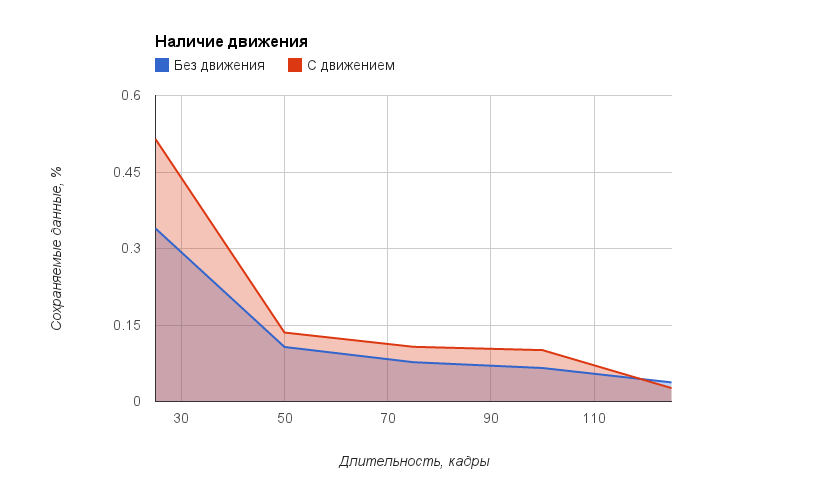
\includegraphics[scale=0.6]{inc/graphics/image1.png}
  \caption{Степень сжатия видео в зависимости от количества движения на видео}
  \label{fig:img1}
\end{figure}

В результате эксперимента было обнаружено, что степень сжатия видео без движения превосходит степень сжатия видео с движением.

\section{Степень сжатия видео в зависимости от количества однотонных областей на видео}

Для оценки зависимости степени сжатия видео от количества однотонных областей с помощью разработанного метода были выбраны два типа файлов. 
Это видео, содержащие реальную съемку, и видео содержащие мультипликацию. Оба типа видео были выбраны без движения.
Мультипликация содержит большее количество однотонных областей, так как при раскраске кадра часто используется заливка. 
Реальная съемка содержит большое количество мелких деталей, что вызывает необходимость сохранять большее коичество коэффициентов после применения 
вейвлетного преобразования для сохранения границ.

Ожидалось, что мультипликация позволит сильнее сжать видео, вейвлетное преобразование имеет преимущество при наличии большого количества однотонных областей на кадре.
В выбраных видео нет движения, не происходит смен сцен, поэтому размер блока не влияет на степень сжатия при выборе одинакового значения для обоих типов видео.
Наличие большого количество однотонных областей позволит удалить большее количество коэффициентов, полученных после вейвлетного преобразования.
Было проведено сравнение видео файлов, отличающихся по длительности и разрешению. Для файлов с одинаковым разрешением, но различной длительностью, было расчитано
среднее значение степени сжатия.

График зависимости процента сохраняемых данных от наличия мультипликации для видео без движения представлен на рисунке \ref{fig:img2}.

\begin{figure}[ht]
  \centering
  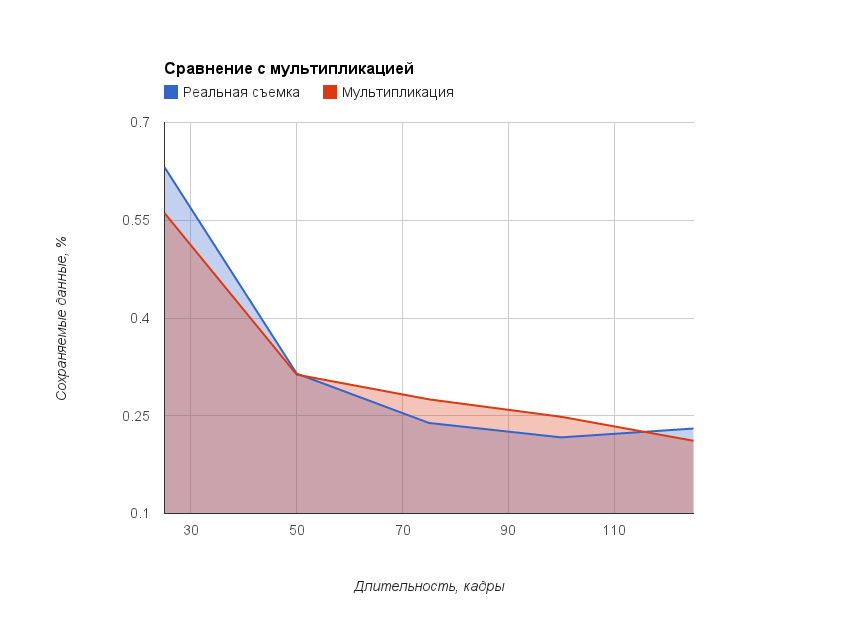
\includegraphics[scale=0.6]{inc/graphics/image2.png}
  \caption{Степень сжатия видео в зависимости от количества однотонных областей на видео}
  \label{fig:img2}
\end{figure}

В результате эксперимента было обнаружено, что мультипликация не дает увеличения при сжатии. Это объясняется тем, что 
современные мультипликации становятся все более похожими на реальную съемку, так как при создании мультипликаций все чаще используются
средства вычислительной техники, позволяющие создавать фотореалистичные изображения. Растет количество деталей на каждом кадре, увеличивается количество границ на кадре.
Это не дает преимуществ при использовании вейвлетного преобразования.

\section{Степень сжатия видео в зависимости от цветовых характеристик видео}

Для оценки зависимости степени сжатия видео от цветовых характеристик видео с помощью разработанного метода были выбраны два типа файлов. 
Это видео, представленные с помощью цветовой модели RGB, и те же видео после удалении информации о цвете.
Видео в градациях серого содержат большее количество смещных пикселей с одинаковым значением, чем видео с подробной информацией о цвете.
При переводе видео в градации серого смежные пиксели, отличающиеся цветом, но имеющие одинаковую яркость, имеют одинаковое значение.
вейвлетного преобразования.

Ожидалось, что отсутсвие информации о цвете позволит сильнее сжать видео, так как вейвлетное преобразование имеет преимущества при наличии большого количества однотонных областей 
на кадре.
В выбраных видео одинаковое количество движения, поэтому размер блока не влияет на степень сжатия при выборе одинакового значения для обоих типов видео.
Было проведено сравнение видео файлов, отличающихся по длительности и разрешению. Для файлов с одинаковым разрешением, но различной длительностью, было расчитано
среднее значение степени сжатия.

График зависимости процента сохраняемых данных от цветовых характеристик видео представлен на рисунке \ref{fig:img3}.

\begin{figure}[ht]
  \centering
  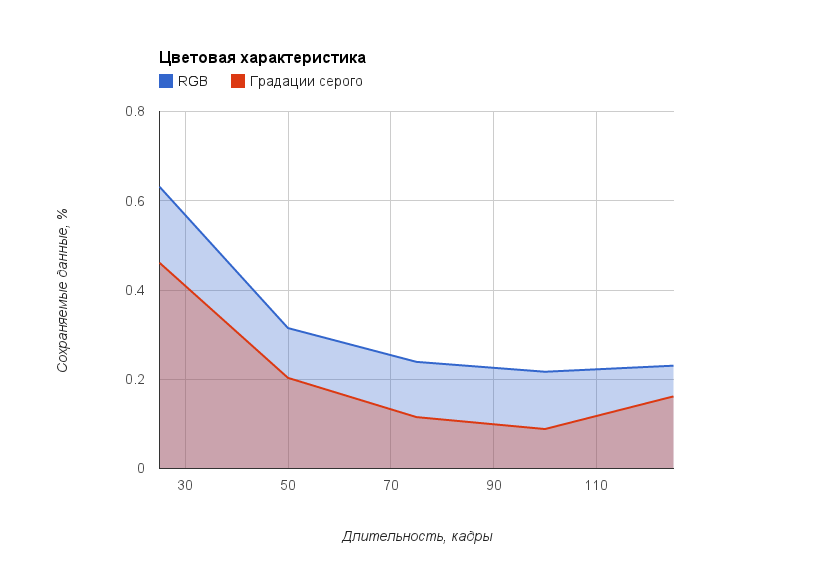
\includegraphics[scale=0.5]{inc/graphics/image3.png}
  \caption{Степень сжатия видео в зависимости от цветовых характеристик видео}
  \label{fig:img3}
\end{figure}

В результате эксперимента было обнаружено, что отсутствие информации о цвете позволяет повысить степень сжатия. 

\section{Анализ результатов экспериментов}

В результате экспериментов были определены типы графических данных, применения к которым разработанного медода дает большую степень сжатия.
Результаты экспериментов представлены в таблице \ref{tab:tres}. Было определено, что разработанный метод имеет преимущества при применении к видео,
имеющим наименьшее количество движения, наименьшее количество информации о цвете и наибольшее количество однотонных областей.

\begin{table}[ht]
  \caption{Анализ результатов экспериментов}
  \begin{tabular}{|p{4.5cm}|p{4.5cm}|p{4.5cm}|}
  \hline
  Характеристика $M$ & Преимущественный тип данных & Причина \\
  \hline
  Количество движения $V$ & Видео без движения & Отсутствие движения в блоке позволяет использовать избыточность данных в глубину \\
  \hline
  Количество однотонных областей $S$ & Не выявлен & Современные мультипликации становятся близки к реальной съемке \\
  \hline
  Цветовая характеристика $C$ & Видео в градациях серого & Пиксели разного цвета близкой яркости при удалении цветовой информации близки по значению, образуются однотонные области \\
  \hline
  \end{tabular}
  \label{tab:tres}
\end{table}